%!TEX program = pdflatex
% Full chain: pdflatex -> biber/bibtex -> pdflatex -> pdflatex

\documentclass[lang=en, 12pt, a4paper, cite=super, chinesefont=Mac-default]{elegantpaper}

%\usepackage{../sub/mystyle_general}
\usepackage{../sub/mystyle_article}
\usepackage{../sub/threeparttable}

% Font
\usepackage[T1]{fontenc}
\usepackage{lmodern}

% Title
\title{Parental Influences on Adolescents’ Physical Activity: Emotional Support, Parenting Style, Parental Engagement, and Gender Differences}
\author{Zhengqing ZHOU \thanks{Peking University} \\ Peking University \and Zhengqing ZHOU \\ PA Technology}
\institute{\href{https://pe.pku.edu.cn/}{Department of Physical Education}}

\version{0.10}
\date{\today}

\usepackage{setspace}
\usepackage{amsmath}
\usepackage{amssymb}
\usepackage{graphicx}
\usepackage[utf8]{inputenc}
\setlength{\parskip}{0.125in}%段间距
\usepackage[autostyle]{csquotes}

% Packages for automated tables
\usepackage{tabularx}
\usepackage{standalone}
\usepackage{pdflscape}
\usepackage{iftex, fancyhdr, hyperref, enumitem, fancyvrb, hologo, multirow, booktabs, bigstrut, tabularx, tocloft}
\usepackage{changes} %批注
\hypersetup{colorlinks = true, allcolors = blue}
\setlength{\hfuzz}{4pt}
\setlist{nolistsep}

% cmd for this doc
\usepackage{array}
\newcommand{\ccr}[1]{\makecell{{\color{#1}\rule{1cm}{1cm}}}}
\addbibresource[location=local]{reference.bib} % reference file
\usepackage{sectsty}
\sectionfont{\large}
\subsectionfont{\normalsize}
\subsubsectionfont{\normalsize}


\begin{document}
{\fontfamily{cmr}\selectfont
\clearpage
\maketitle
\thispagestyle{empty}

\begin{abstract}
{\fontfamily{cmr}\selectfont
Background/Purpose: Adolescent physical inactivity likely contributes to global health problems. Despite the parents played an essential influence on adolescents’ physical activity (PA) has been proved a lot, few studies have explored the different characteristics of parental influence on adolescents’ PA. The purpose of this study was to examine the relationship between parental influences and adolescents’ PA by gender.

Methods/Design: Data are from the first wave of the China Education Panel Survey in 2013-2014. The sample includes 5976 youth (51.6\% in grade 7), 3046 are female, and 2930 are male. The PA level of the adolescents was measured using total minutes on weekdays. The influences of parents, including emotional support, parenting style (responsiveness and demandingness), and parental engagement, were measured by the average scores of a count of questions. For adolescents with both a mother and father, the scores were averaged across the two parents.

Results: Parental influence had a positive impact on adolescents’ PA for both genders in general (coefficients and 95\% confidence intervals for females, 0.17 [0.10-0.23] and males, 0.15 [0.10-0.21], respectively). More specifically, emotional support, parenting style, responsiveness, and parental engagement also positively influenced PA (coefficients and 95\% confidence intervals for females, 0.24 [0.18-0.29], 0.04 [0.01-0.06], 0.48 [0.19-0.76], 0.89 [0.56-1.22], and males, 0.20 [0.15-0.26], 0.03 [0.01-0.06], 0.45 [0.22-0.68], 0.45 [0.16-0.74], respectively); However, demandingness did not. Besides, Father and mother generated different influences in adolescents of different genders. All the results above are obtained after controlling covariates and fixed effects and clustering in school and grade.

Conclusion: Strategies to promote physical activity among adolescents should focus on increasing levels of parental emotional support, parenting style, parental engagement, and playing different parental roles on adolescents of different genders.

    \par
\keywords{Elegant\LaTeX{}, Working Paper, Template}
}
\end{abstract}

	\newpage
    \phantomsection
    \addcontentsline{toc}{section}{摘要}
    \tolerance=500 %将摘要放进目录
    \tableofcontents
    \setcounter{page}{1}
	\newpage

% Update Notes
	\newpage
    \section*{Update Notes} 
    \label{Update Notes}
    
    • Topic and Variable 
    
    • Which One  
     
    • follow Bobby W. Chung \& Jian Zou

    Step 1:
        
    We utilize random assignment of students into classrooms in China middle schools to study the mechanisms behind the spillover of peer parental education on student achievement. 
    
    Analyzing the China Education Panel Survey, we find a    causal relationship between X and Y. 
    
    In addition to the conventional peer effect and teacher response channel, we identify mother adjustment of parenting style as another important mediating factor. 
    
    find W as mediating factor.
    
    We provide suggestive evidence about the existence of the mother’s network, which facilitates the change in parenting style. 
    
    We also find that the spillover of peer maternal education on non-repeaters and non-migrant students is stronger, primarily driven by higher parental investment in time.
    
we follow the method by Gong,Lu, and Song(2018), which is classroom assignment randomization. Our selected sample is almost identical to that of Gong, Lu, and Song (2018).

Our Y is PA , measured by the question:

In the raw data, the scores of the three subjects have been standardized with a mean of 70 and a standard deviation of 10. Then we generate the standardized PA timing with a mean of 0 and a standard deviation of 1.

Throughout this paper, groups are defined as migrant and local students. in each one, there are 11111 students on average, and in each class per group with a minimum of 21 and a maximum of 81.

The key variable of interest are three: one, Social Integration (assi); two, class diversity with some characters (made of an index); three, check the character of parents.
% Section
	\newpage
	\section{Research Questions} 
	\label{Research Questions}
	\subsection{SI and PA}
Q1. does Social Integration affect PA?

A1. possitive 

Hypothesis 1: All other variables being equal, the higher the Social Integration of children, the more time they will spending time on physical activities. And there is heterogeneity in different groups.


Hypothesis 2: All other variables being equal, diversity in the classroom has an inverted "U" shaped relationship with with the behaviors among adolescents' cross-group friends.

\subsection{Class Divsity and PA}

Q2. does Social Integration affect PA?

A1. ? 

Hypothesis 3: All other variables being equal, The greater the density of cross-group interactions among the groups to which they belong in the class, the greater the number of adolescents' cross-group friends.

Hypothesis 4: The higher the density of homogeneous external group interactions, the lower the number of adolescents' cross-group friends, all other variables being consistent.

\subsection{Migrate and local differences in Class Divsity influences}

Hypothesis 5: There will be significant differences in the effects of group composition of the class, cross-group interaction density of the group to which they belong, and homogeneous interaction density of the external group on the number of cross-group friends of mobile and local children.

通过已有研究可以发现,首先,目前大多数研究对教育获得因果机制的探究中,只有少数对比了不同家庭维度对孩子教育获得成果的影响。其次,国内外的研究更加侧重家庭静态因素对子女教育获得的影响,较少关注家长参与、情感投入等动态因素,而对比这两条不同路径对子女认知能力的影响的研究则更少。在仅有的比较不同类型的教育投资对认知能力影响的研究中,对家庭经济条件的测量则过于简单,未将家庭多元的教育投入纳入考虑,如课外补习花费、校内学习花费等具体经济变量。最后,国内关于学生认知能力的研究大都使用了中国教育追踪调查数据(CEPS)2013-2014年基线数据,而该数据在许多关于教育投入的变量上存在大量的缺失情况,以往的研究中也很少有学者关照到这些数据缺失的情况并对其进行处理。因此,本文以一个动态的视角来比较不同类型的家庭教育投入对孩子认知能力的影响,综合运用不同维度的理论视角作为指导,同时也采取更细化的指标及完整的数据进行研究,以期能更加科学和严谨。
% Introduction
	\newpage
	\section{Introduction} 
	\label{Introduction}
	定期参加体育活动(PA)对于维持整个生命周期的健康和福祉至关重要。大量证据显示在儿童和青少年中,身体活动可以显著改善身体健康(心肺和肌肉健康)、骨骼健康、认知结果(学业成绩和执行功能)、心理健康(抑郁症状机减少)以及肥胖症状减轻(WHO,2020),但在发展中国家,许多儿童仍旧无法得到充足的锻炼。当前,中国青少年的心理健康问题不容忽视。据估算,约7%~30%的中学生存在焦虑、抑郁等心理健康问题。数据显示......这一现象也引起中国政府高度重视,《“健康中国2030”规划纲要》提出要实施青少年体育活动促进计划,培养青少年体育爱好。

青少年缺少PA的一个重要的原因是其复杂、多样的决定因素,包括个人、家庭、学校和社会等多种环境因素会影响儿童和青少年行为(Biddle和Asare,2011年;Mitchell等人,2016年)。近30年的改革开放,中国一方面经历了快速的城市化和工业化发展,另一方面见证了时间最大规模的流动人口。城乡间大规模的人口流动为中国城市发展带来充足的人力和智力支持,同时也使得流动人口与本地居民的社会融入问题日益突出。事实上,这种社会空间的隔离也进一步导致流动儿童面临较为严重的城市融入问题。并且在心理发展、教育期望、学业表现等方面与本地儿童相比均处于明显的劣势(周皓、巫锡炜,2008;柳建坤等,2020;谢建社等,2011)。因此,分析和考察流动儿童和本地儿童的社会融合对青少年的健康发展、促进教育公平和城市社会的可持续发展具有重要的现实意义。为了改善家庭经济状况和生活质量,大量农村劳动力选择进程务工,同时子女也随父母远离家乡,成为了流动儿童。

作为青少年行为中啊哟关于流动儿童其父母影响运动参与问题,目前的研究或者直接分析影响流动儿童社会融入的现实障碍和影响因素。不可否认,这些研究对于我们理解流动儿童的社会融入问题具有重要意义,但它们大多忽视了流动儿童社会融入过程中的另一个重要问题——社会交往,更确切地说,是流动儿童与本地儿童之间的友谊问题。学校和家庭是青少年日常生活中最为重要的两个生活场域。学校不仅为青少年提供了适应未来工作和生活所必备的知识和技能,也同时为他们建立同伴关系和发展友谊提供了一个相对制度化的社会交往空间。然而,不同学校,甚至学校中不同班级之间,在群体构成、同辈互动情境等方面往往存在显著差异。因此,青少年在不同的学校和班级所面临的社会交往环境可能会完全不同,进而发展出迥异的社会交往关系(McFarland,etal.,2014)。更进一步说,这种社会交往关系还可能会因为青少年社会身份(如流动儿童和本地儿童)的差别而存在较为明显的差异。同样,作为社会化的另一个重要场所,家庭也对青少年的社会交往有重要影响。不同阶层的父母所持有的价值观念以及亲子间互动的方式都会潜移默化地影响青少年社会交往的方式和偏好(VanTubergenandSmith,2018)。,却只有少量国内学者注意到这一问题(史晓浩、王毅杰,2010;王毅杰、史晓浩,2010),而且也没有进行严谨的实证检验。

基于此,本文旨在考察同伴效应对青少年体育锻炼是否构成因果关系。基于国内范围最广的教育追踪调查数据,笔者使用工具变量方法消除了潜在的同伴效应内生性问题,发现同伴效应对初中生的体育锻炼时间具有正向显著影响。同时验证了了王富百慧等(2018)以及权小娟和卢春天(2020)的假设,即同伴支持同样会对个体锻炼时间有显著正向促进作用。进一步机制分析发现,班级运动氛围在同伴效应影响青少年体育锻炼时间路径中起中介作用,一方面同伴效应会显著正向促进班级运动氛围提升,另一方面,班级运动氛围同样提高个人运动参与。

综上所述,本文边际贡献主要体现在两个方面:首先,在理论上将青少年个体运动行为与教育学中经典的同伴效应问题进行连接,呼应Manski(1993,2000)等学者指出的内生性问题对同伴效应估计中造成的偏误影响,揭示了本领域研究“重相关,轻因果”传统而常忽略的遗漏变量问题。其次,实证方面,建立在教育追踪调查的数据优势允许我们使用基期调查时的同伴数据作为同伴效应的替代测量,同时将基期同伴父母的运动陪伴作为当期同伴效应的工具变量,获得了同伴效应的纯净估计值。最后,对同伴效应影响青少年体育锻炼行为的机制深入分析,班级运动氛围中介效应能够解释近20\%的总效应影响,该结论不仅从再次从学理层面验证了同伴效应对青少年体力活动促进的重要性,而且为从实践层面为合理引导学生参与体育锻炼提供了政策启示。

余下的部分安排如下,本文的第二节是文献回顾,第三节是研究设计,第四节是数据来源与数据描述,第五节是研究结果与分析,最后给出本文的结论和政策建议



基于上述讨论,本研究将着重检验当前中国初中教育阶段家庭背景和学校的班级情境对流动儿童和本地儿童之间跨群体交往的影响差异。具体来讲,通过分析“中国教育追踪调查”(CEPS)数据,本文试图回答以下问题:第一,家庭社会经济地位对青少年的跨群体交往的影响和群体差异;第二,班级情境,尤其是班级中的群体构成、同辈群体、外部群体对青少年的跨群体社会交往起到何种作用,以及对流动儿童和本地儿童又有何种差异虽然这些流动儿童会与父母生活一起,但让他们受父母工作、家庭环境等因素变化,对校园活动那个产生影响。家庭、学校和社会是儿童青少年进行体育运动的三个主要场域,其中家庭是个人社会化最初的场所,家庭教育是学校教育和社会教育的基础,大量研究已经证明,在早期的体育兴趣培养中,家庭相对于学校和社会的影响是最大的。家长的期望信念、价值信念与子女的教育期望会与PA呈高度正相关。家长对子女要求越高,与教师越匹配就荣促进参加PA。家长与子女的互动越多,对PA有正向作用。行为,家长行为会诱导孩子模仿。家长的社会资本越多,孩子可能会承接家长的交流能力,从而促进PA。同伴的家长特征,就会促进PA。比如同学的家长,陪同孩子参加课外体育锻炼、家长经常与孩子一起娱乐,都会促进孩子参加体育锻炼。中介方面,认可度较高的家长教养方式、家庭社会资本、家长教育程度、家庭经济条件也是显著因素。家庭体育是青少年行为养成的重要依托。父母作为家庭主要成员,对青少年体育锻炼参与度有广泛的影响。然而,青少年在行为养成时期,家庭因素影响占比逐渐增大。因此这一时期要格外注重家庭体育环境的建设和优化。

% Data and Measurement
    \newpage
    \section{Data and Methods} 
    \label{Data and Methods}
    \subsection{Data}

According to Manski (1993), the use of a randomly assigned sample is necessary to remove the group factor of interest from the correlation effect, so this paper selects a "randomly assigned" sample of schools in which new students are randomly assigned at entry and are not reassigned thereafter, nor are they assigned to classes based on any course subject scores.

近些年不少文献也使用该数据中的随机分班样本进行教育学研究(Gong et al.,2018,2021;Hu,2018; 李长洪和林文炼,2019 等等)。

This study primarily uses CEPS baseline survey data from 2013-2014. School data are often self-selective, i.e., students are assigned to specific classes due to potentially observable or unobservable factors, which can lead to bias in estimating the educational production function. Ideally, in this study, individual student characteristics and classroom characteristics would not affect the class assignment outcomes, i.e., students would be randomly assigned to different classes. Although the Compulsory Education Law of the People's Republic of China strictly requires that junior high schools should not divide their schools into priority and non-priority classes, some schools may not strictly adhere to this rule in practice. {For this reason, the following steps were used to screen schools that may not strictly adhere to the random assignment rule.} First, each principal was asked to respond to two questions about whether 7th graders were randomly or equally assigned to classes upon entry, and whether these students would be reassigned to classes later in secondary school (i.e., in 8th and 9th grades). Schools that reported non-random assignment of students in grade 7 or reassignment in grades 8 and 9 were excluded from this study. Second, classroom teachers were asked to report whether students were assigned based on test scores. Schools whose classroom teachers reported being assigned by performance were also dropped from this study. Finally, the sample for this study includes approximately 10,000 students in grades 7 and 9 from 256 classes in 64 schools.

The key variable of interest is the educational background of peers' parents. We measure it by the average college attainment of classmates’ mothers and fathers separately. To avoid spurious correlation, we follow the approach by Moffitt et al. (2001) to calculate the ‘leave-me-out' average. We use pre-determined variables of students to implement balancing tests for the random assignment and include them as controls in the main specifications. The control variables include age, gender, ethnicity, rural status, local residency status, only child indicator, whether one attended kindergarten, student's age attending primary school, whether one repeated Or skipped in primary school, non-cognitive measures, and parental college education attainment. In Table 1, we provide summary statistics for the aforementioned variables.a

Data are from the Behavioral Risk Factor Surveillance System, a large nationally representative telephone survey of the non-institutionalized adult population administered by the Center for Disease Control and Prevention. Between 2001 and 2005 all states participated. We drop any pregnant women from the analysis as physical activity recommendations are dependent on prior physical fitness. Annual sample sizes range from approximately 112,000 to over 258,000 leading to a combined sample size of over 1 million observations when all four years are used.

概念界定:此前,学术界对流动儿童的概念没有统一、权威的定论。学者周皓将流动儿童的概念界定为6—14周岁且随父母或其他监护人在流入地暂时居住半年以上的儿童少年,又称“流动人口子女”、“进城务工人员子女”等。流动子女与留守子女。相对应。学者范先佐认为流动儿童是指跟随父母移居城市上学的进城务工就业的农民子女,与父母进城务工就业而将子女留在老家的“留守儿童”相对应本研究对农村大龄流动儿童界定有以下两方面限制:1.正在接受初中阶段义务教育的儿童、2.来自农村,且与父母同住。本研究在界定目标人群时,首先依据户籍类型、是否流动两项变量,再根据对农村大龄流动儿童的界定,从整体样本中抽取出2130名拥有农业户籍、跨省及省内流动的流动儿童,其中男性、女性流动儿童分别有1125名、1005名;抽取了7455名拥有城市户籍、没有流动经历且与父母同住的城市儿童,其中男性、女性城市儿童分别有3777名、3678名。(一)不同生活环境的儿童、不同性别流动儿童主观幸福感的差异(二)农村大龄流动儿童主观幸福感的相关影响因素

\subsection{Measurement}

For the non-cognitive measures: CEPS asks students seven questions on personality traits at Grade 6. The first three questions measure persistence, while the rest measures other personality traits. We follow the approach by Zou (2020) and Gong, Lu and Song (2018) to obtain a “persistence” index by averaging the responses of the first three questions and a “other non-cognitive” measure by averaging the responses of the rest four.

被解释变量:本研究衡量学生行为的主要指标是学生体育锻炼时间。体育锻炼是影响青少年健康的重要因素,比如(Y2),甚至会影响接受人力资本的形成。

其中,认知技能是用学生期中考试的三门主课成绩和 CEPS 提 供的标准化认知能力考试成绩来衡量。学校的行政办提供了学生三门核心科目 (语文、数学和英语)的期中考试成绩。学业成绩是学生未来社会经济状况的一个非常重要的预测因素,尤其是初中阶段的学习成绩,直接决定着他们进入高中 和大学的可能性和质量。

认知与非认知技能都是影响学生未来发展的重要因素,比如影响学生接受高等教 育的机会和劳动力市场的结果(Heckman and Rubinstein,2001;Heckman et al, 2006 and 2013)。

解释变量:
本研究的关键解释变量有两个(X1-X5)

父母情感投入维度:情感投入是指在一项活动或者事物中,全身心地投入,并且感情深深地投入其中。这可能是一项艺术活动,如阅读、写作、画画或音乐,也可能是一项爱好,如运动或兴趣爱好。情感投入也可以指在工作或与他人相处方面的投入。情感投入是一种积极的心态,它能帮助人们更加全身心地投入活动,获得更多的乐趣和满足感。指标表现在:对子女以下问题的关心:

教养风格(PS):



其一是学生个人是否接受过学前教育,这是一个虚拟变量(是,赋值为 1);

其二是班级中接受过学前教育的学生的比例。 CPES学生问卷中咨询学生 3 岁以后有没有上过幼儿园/学前班?这里将回答为 “是”的学生赋值为 1;回答为“否”的学生赋值为 0。
【进一步,将这个变量汇总到班级层面,计算出每一个班级中每位学生除了自己之外的班级中接受学前教育的学生占比。】

在具体的操作中,首先生成每个人是否接受学前教育的虚拟变量,然后得到班级中学前 教育的学生占比(除自己之外),此时得到的这两个核心解释变量的均值应该是一致的。


如前所述,已有的各种研究表明,早期人力资本投资对认知和非认知技能在青年期和成年期的成长有极其重要的影响(Almond et al.,2018;Currie and Almond,2011;Cunha and Heckman,2007)。最近的一项研究为本文提供了支持,Cornelissen and Dustmann(2019)利用英国小学独特的入学规则,来识别和 估计学前教育的因果效应。他们发现了学前教育的持久影响,接受过学前教育的 学生通常比没有接受过的学生在智力和情感发展方面表现得更好;随着年龄的增长,学生表现出更高的学习兴趣并且在课堂上表现出较少的破坏性行为(例如破坏课堂纪律或对同学产生的暴力行为)。【进一步,他们还发现处境不利(家庭困难)的男孩从学前教育中受益最大,这可能是由于学前教育为男孩提供了比家中更为健康的环境。】Cornelissen and Dustmann(2019)的研究表明,接受过学前教 育的学生通常拥有更强的能力;那么如果班级中接受学前教育的学生越多,整个 班级的平均人力资本存量就会越高。如果不同班级的平均人力资本存量存在随机 性的差异,这种差异是否会影响不同学校和班级的学生的人力资本发展呢?

parenting style是指家长对于育儿的具体方式和理念。家长可能会采取不同的育儿方式,这些方式可以归纳为四种主要的育儿风格:权威型、宽容型、放任型和严厉型。权威型育儿风格是指家长对孩子实施科学、合理的管教方式,同时也尊重孩子的个性和独立性;宽容型育儿风格是指家长尊重孩子的意愿,允许孩子自由选择和实现自己的目标;放任型育儿风格是指家长缺乏约束和管教,不加干预孩子的行为;严厉型育儿风格是指家长高度控制孩子的行为,采取严格的惩罚措施。不同的育儿风格可能会对孩子产生不同的影响,家长应根据孩子的特点和需求,选择最适合孩子的育儿方式。

控制变量:
个体特征控制变量:性别(女生=1)、民族(汉=1)、同胞数量、户籍类型(农村=1),这些变量属于事前变量

班级特征控制变量:班级规模、班级性别组成、班级的学生家庭经济状况、班主任年龄、性别和班主任职称



\subsection{Statistical analysis}



% Estimation Strategy
    \newpage
    \section{Estimation Strategy}
    \label{Estimation Strategy}
    \subsection{Class Assignment and Regression Sample}

为验证样本“随机分班”的可靠性,我们分别从学生和教师特征进行检验。 表 3-2 从全样本和分年级样本检验学生个体先决特征变量与班级其他同学特征 的相关性。借鉴 Sacerdote et al.(2001)、Guryan et al.(2009) 和 Eisenberg(2014) 的 随机检验方法,如果学校内部随机分班的假设成立,在控制学校年级固定效应 后,个体的先决特征变量和同伴的平均特征无关,即个体的先决特征变量对同 伴该变量的均值做回归,其回归系数应该不显著。Guryan et al.(2009) 指出在样本有限的情况下,该检验存在固有偏差,因为个体不可能是自己的同伴,即使 在随机分配的样本中,个体的先决特征变量和同伴的平均特征也出现显著的负 相关。比如一个高能力个体的同伴能力要比低能力个体的同伴能力更差。而如 果回归中出现显著的正相关,则表明学生在班级之间存在相似的学生被分配到 相同班级的现象,随机分班的假设不成立。

表 3-2 中列出了分别以个体每个背景特征为因变量,对同伴相应的先决特 征变量的均值进行回归的系数。结果显示个别变量(全样本中的学生性别、母 亲教育水平和父亲职业、九年级中的农业户口)存在系数显著且为负的情况, 大部分变量的系数不显著,没有出现正向显著相关的情况。根据 Guryan et al.(2009) 指出的在样本有限的情况下,这些负相关属于随机检验中存在的固有偏 差。因此总体上看,并没有发现学生与其同伴特征有显著的正向选择问题。 为检验教师是否随机被分配到每个班级,表 3-3 汇报了控制学校年级固定 效应后,班主任的每个先决特征(班主任性别、班主任教学经验、班主任学历 和班主任年龄)对班级学生和其父母的每个背景特征的均值分别进行回归的系 数。结果显示回归系数都不显著,表明在随机分班的学校样本中,教师特征与 班级学生和其父母特征之间并不存在显著的相关性。


因果推断的有效性依赖于随机分班的可靠性。鉴于学生家庭背景特征是影 响学生行为表现的重要因素,我们在表 4-3 中分别用因变量对除了班级高能力 学生比例以外的其他学生个体、家庭背景特征和班主任特征先决变量进行回归, 同时控制学校年级固定效应。回归结果表明学生性别、父母的教育水平、家庭 经济状况等变量显著影响学生的认知和非认知能力。在确认了影响学生行为表 现的先决变量之后,为了估计随机分班的可靠性,我们借鉴 Xu et al.(2020) 的随 机分班检验方法,用班级高能力学生比例对普通学生的个体和家庭背景特征先 决变量进行回归来检验随机分班的可靠性。如果随机分班被严格执行了,那么 学生个体和家庭背景特征先决变量和高能力学生的比例不相关,其回归系数应 该不显著。该结果呈现在表 4-3 的第(5)列,结果显示,除了学生性别和班主 任学历外,其他先决变量的系数都很小并且都不显著。因此尚未发现学生被分 配到高能力学生比例较高班级的可能性。 另一种验证样本“随机分班”可靠性的方法是从学生和教师两个方面进 行随机分班检验。我们借鉴同样使用 CEPS 随机分班样本数据的 Gong et al. (2018,2021) 中平衡性检验(balancing tests)的方法,如果随机分班假设成立, 班级中高能力学生的比例与普通学生个体背景特征和教师特征的先决变量(如 户口类型、独生子女、父母教育水平、家庭经济状况、任课老师的性别、年龄、 学历、教龄等等)无关。

因此,表 4-4 中列出了基于学校年级固定效应模型分别以普通学生的个体 背景特征和教师特征为因变量对班级高能力学生比例进行回归的系数。从表 4-4 中第一列的检验学生是否随机被分配到每个班级的回归结果看,在相同学校相 同年级中,除了学生性别、上过幼儿园和小学留过级变量以外,高能力学生的 比例与普通学生个体和家庭背景的大部分特征都没有显著的关系。

个别变量在组间有显著性差异在研究同伴效应文献的随机分班平衡性检验中并不少见,如:Gong et al (2018, 2021)、 Wang et al (2018)、 Lavy et al (2012)、 Carrell et al.(2013) 和 Carrell et al.(2010) 等等。从表4-4中第二列的检验教师是否随机被分配到每个班级的回归结果看,回归系数几乎都不显著,表明在随机分班的学校样本中,教师特征与班级学生特征之间并不存在显著的相关性,我们可以排除学校分配更好的老师给高能力学生比例更高班级的可能性。因此, 我们可以基本证实随机分班的可靠性。

\subsection{Methodology}

根据前述研究假设,本文仍采用传统线性均值模型,并扩展了Ryan(2017)的方法四,将基准模型设定为方程\eqref{eq:basic.reg}来验证班级中的同伴效应对初中生体育锻炼行为的影响。

\begin{equation}
PA_{i,c,s} =\beta_0 + \beta_1 * {ParSty}_{i,c,s}+\beta_2 * {SoG}_{-ics} + \boldsymbol{\gamma} \boldsymbol{X}_{i,c,s} +\boldsymbol{\gamma}\boldsymbol{P}_{i,c,s}+ \omega_g+\lambda_s+\delta_{gs}+\varepsilon_{i,c,s}
\label{eq:basic.reg}
\end{equation}

where Y.ih refers to the test score of student i in class i in a school-grade k. Mother Ed.n元, is the leave-me-out average college attainment of mothers in a classroom. Xi,k is a vector of control variables listed in Table 1.8 We isolate the effect of teacher characteristics (TY,k, On students by including head teachers’ age, gender, marriage status, whether having a college degree, teaching experience in years, whether graduated from a normal college, and whether having a teacher certificate (Gong, Lu and Song, 2018).

We include school-by-grade fixed effect (x) to control for school and residential sorting.

With the fixed effect, the variation of Mother Edu-ii,h then entirely comes from within-grade classroom composition, which is the level the randomization happens. Our randomization setting is rare and unique, especially with a national sample of students. An analogous dataset in the US is the National Longitudinal Study of Adolescent to Adult Health (Addhealth), which contains actual friendship detail for a national sample of US students and is widely used in the peer effect iterature. Because of the concern over individual sorting into peer groups, researchers require additional assumptions to identify the spillover of peer parental education (Bifulco, Fletcher and Ross, 2011; Bifulco et al., 2014; Olivetti, Patacchini and Zenou, 2018; Chung, 2020).

\subsection{Balance Test}

这部分包含:平衡性检验

因此,本研究借助 CEPS 数据特有的分配规则,将样本限制在那些随机分 配学生的学校,以此来解决潜在的内生同伴选择问题。研究的关键识别假设是, 学生是被随机或者平均地分配到班级中去。为此,首先按照第二节中提供的分配 规则信息,识别出本研究的样本;然后进一步利用统计性检验来验证这一随机分 配假设的有效性。 具体而言,这里采用两个统计性检验。第一个统计性检验一般被称为平衡性 检验(Balancing test)38。在具体的回归分析中,将第二节中提到的个体层面的 事前控制变量对班级中受过学前教育的学生占比进行回归;以及将班级层面的控 制变量对个人是否接受学前教育进行回归。如果学生在一个学校里被随机分配到 任意班级,那么班级中接受学前教育的学生比例变量与那些观察到的、可能破坏 随机分配规则的个体特征之间不应该存在统计相关性。同理,如果学生是被随机 分配的,那么个人是否接受学前教育这一事前变量,也不会与班级层面的变量有 关联。举例而言,假设接受过学前教育的孩子的父母,他们更重视人力资本投资, 因此希望孩子可以进入某个名师的课堂,或者说会选择让孩子进入有某种家庭背 景的学生聚集的班级,那么就可能看到个人是否接受学前教育这个变量就会与那 些班级层面的变量显著相关。所以,如果上述回归结果中存在较多变量的估计系 数在统计上显著,就表明此样本数据违反了随机分配假设,而估计结果也将存在 偏误。

Before we estimate the spillover of peers’ maternal education, we verify the peer group assignment is as good as random. Because our identification relies on within-grade variations of classroom composition, we need to make sure there are ample variations of the treatment variable.

图1a显示了X变量在各班级中的原始分布,其中x轴代表班级标识符,y轴代表班级中X比变量的比例。我们在图1b中进一步将这些数值组织成柱状图。如图所示,班级中拥有X变量从0到63.64个百分点不等。在图2a中,我们显示了在同一学校年级的条件下,不同班级间X变量的相关性。每个点代表一个学校年级,X轴是班级1的X的变量比例,Y轴是另一个班级2的X变量。该图的想法是看看两个班级是否相同的数值,在这种情况下,点将正好落在45度线上。如图所示,许多点都是分散的,这意味着即使控制了按年级的固定效应,我们的处理变量也有很大的变化。在同一硬币的另一面,图2b描绘了大学毕业的母亲比例的年级内班级间差异的柱状图。差异范围从0到28.30个百分点,超过60%的班级对没有相同的值。这再次表明,我们的处理变量有足够的变化来进行识别。!!

作为本文最重要的识别手段,下文将继续对上述52所样本学校的“随机分班”特征进行检验。具体来说,本文根据同校内的两个班级设定虚拟变量,进而考察其与学生在7年级时的心理健康状况及其他个人、家庭、父母、班级和学校特征之间的关系,回归结果见表2。可见,几乎所有基线变量都不与班级虚拟变量存在显著关系①,这在一定程度上支持了样本校的分班随机性。

在对样本校的随机分班特征进行检验后,另一个需要注意的问题是,学校在各班级之间的资源分配是否平衡。例如,为完成某些教学目标,学校可能在随机分班后对某班级投入更多的教育资源。因此,参考王海宁等的研究(Wangetal.,2018),本文将继续考查学生及其家庭可观测特征的班级均值(例如学生年龄、性别、民族、出生次序、兄弟姐妹数量、户口、家庭经济条件及父母受教育年限)与班级和教师特征(例如班级规模、教师个人特征及行为特征)之间的关系,回归结果见表3。根据检验结果,在加入学校固定效应的条件下,几乎所有系数都不显著(仅存在四个例外,但是估计值均较小且可能来源于样本误差)。可见,对于随机分班的样本校,其在校内各班级之间的资源分配也没有表现出显著倾向。

我们还通过观察LBC在学校和年级中的比例变化是否与几个预定的学生特征的变化有关,来研究识别策略的有效性。如果这个分配过程是真正的随机的,那么学生在这些预定的特征上应该是相似的[29]。我们分别进行回归,其中因变量是学生的预定特征,而班级中LBC的份额是自变量,加入年级和学校的固定效应和学校特定年级的趋势效应。表3中的证据支持上述识别假设的有效性。也就是说,学生的预定特征在具有不同LBCs学生份额的班级中是平衡的。

我们加入了按年级的固定效应(ox)来控制学校和居住地的排序。有了固定效应,母亲Edu-ij.k的变化就完全来自年级内的教室构成,这就是随机化发生的水平。我们的随机化设置是罕见和独特的,特别是在全国性的学生样本中。在美国,一个类似的数据集是全国青少年到成人健康纵向研究(Addhealth),它包含了美国学生的全国性样本的实际友谊细节,并被广泛用于同伴效应文献。由于对个人分类进入同伴群体的担忧,研究人员需要额外的假设来确定同伴父母教育的溢出(Bifulco,Fletcher和Ross,2011;Bifulco等人,2014;Olivetti,Patacchini和Zenou,2018;Chung,2020)。

As an additional check, we performed Monte Carlo simulations for the elementary, middle, and high school samples to verify that the observed within school variation in the proportion of female students was consistent with a random process. For each school, we randomly generated the gender of the students in each cohort and computed the within school standard deviation of the proportion female.17 We repeated this process 1,000 times to obtain an empirical 90 percent confidence interval for the standard deviation for each school.



% Results
    \newpage
    \section{Results}
    \label{Results}
    \subsection{基准回归}
%
%\begin{center}
%\begin{figure}[h]
%\centering
%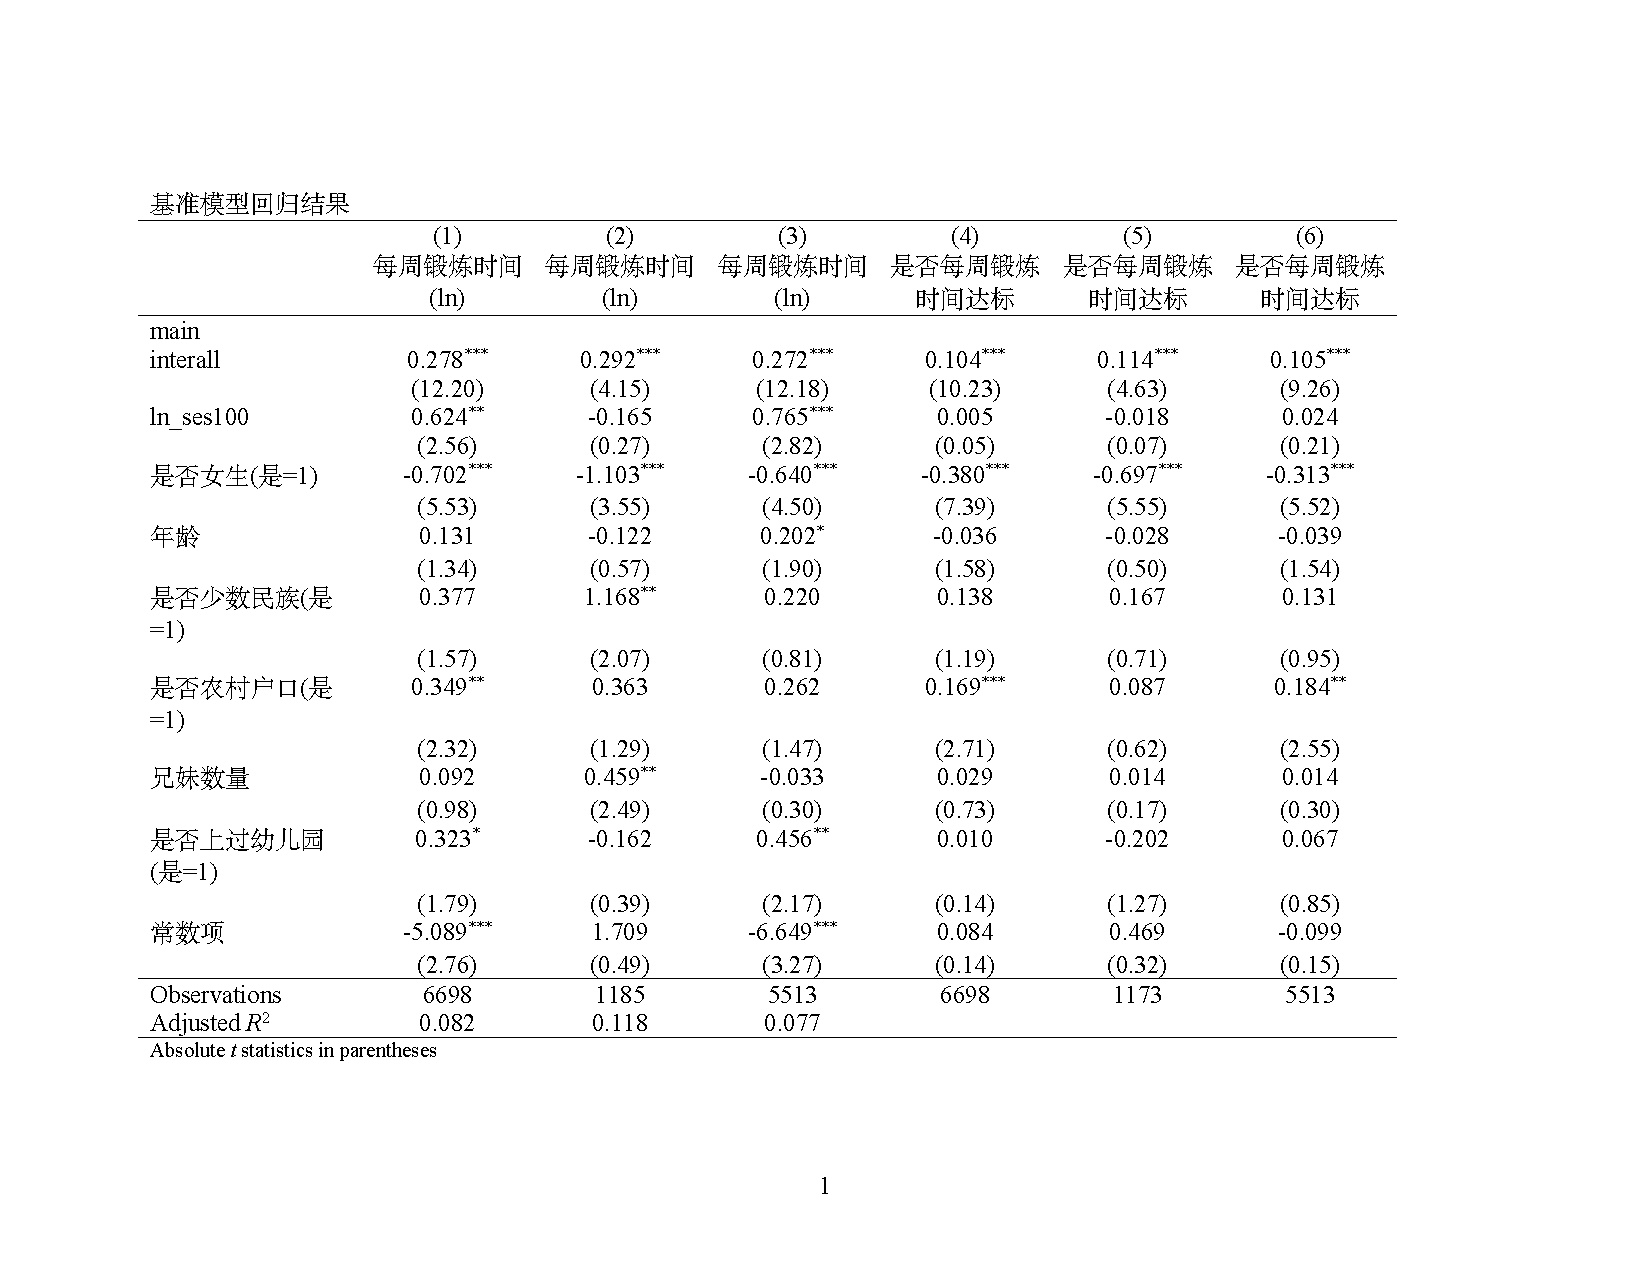
\includegraphics[width=1.25\textwidth]{figures/basigreg01.pdf}
%\caption{基准回归模型}
%\label{fig:}
%\end{figure}
%\end{center}

\subsection{异质性分析}
% Conclusion
	\newpage
	\section{Conclusion} 
	\label{Conclusion}
	\input{./sub/conclusion.tex}
% Appendix
	\newpage
	\appendix
	\section{Appendix}
	\label{Appendix}
	
% FIGURES
\subsection{Figures}

\begin{figure}[H]
\caption{}
\centering
%\includegraphics[scale=1]{../../output/}
\label{fig:}
\end{figure}


% TABLES
\newpage
\subsection{Tables}

\begin{table}[H]
\caption{}
\centering
\begin{threeparttable}
%\input{../../output/}
\end{threeparttable}
\label{tab:}
\end{table}

	
	\newpage
    \printbibliography[heading=bibintoc, title=\ebibname]
    \appendix
%\appendixpage
    \addappheadtotoc

}
\end{document}
